%%%%%%%%%%%%%%%%%%%%%%%%%%%%%%%%%%%%%%%%%
% Masters/Doctoral Thesis 
% LaTeX Template
% Version 2.5 (27/8/17)
%
% This template was downloaded from:
% http://www.LaTeXTemplates.com
%
% Version 2.x major modifications by:
% Vel (vel@latextemplates.com)
%
% This template is based on a template by:
% Steve Gunn (http://users.ecs.soton.ac.uk/srg/softwaretools/document/templates/)
% Sunil Patel (http://www.sunilpatel.co.uk/thesis-template/)
%
% Template license:
% CC BY-NC-SA 3.0 (http://creativecommons.org/licenses/by-nc-sa/3.0/)
%
%%%%%%%%%%%%%%%%%%%%%%%%%%%%%%%%%%%%%%%%%

%----------------------------------------------------------------------------------------
%	PACKAGES AND OTHER DOCUMENT CONFIGURATIONS
%----------------------------------------------------------------------------------------

\documentclass[
11pt, % The default document font size, options: 10pt, 11pt, 12pt
oneside, % Two side (alternating margins) for binding by default, uncomment to switch to one side
spanish, % ngerman for German
singlespacing, % Single line spacing, alternatives: onehalfspacing or doublespacing
%draft, % Uncomment to enable draft mode (no pictures, no links, overfull hboxes indicated)
%nolistspacing, % If the document is onehalfspacing or doublespacing, uncomment this to set spacing in lists to single
%liststotoc, % Uncomment to add the list of figures/tables/etc to the table of contents
%toctotocnumbered, % Uncomment to add the main table of contents to the table of contents
parskip, % Uncomment to add space between paragraphs
%nohyperref, % Uncomment to not load the hyperref package
headsepline, % Uncomment to get a line under the header
chapterinoneline, % Uncomment to place the chapter title next to the number on one line
%consistentlayout, % Uncomment to change the layout of the declaration, abstract and acknowledgements pages to match the default layout
]{MastersDoctoralThesis} % The class file specifying the document structure


\selectlanguage{spanish}

\usepackage[utf8]{inputenc} % Required for inputting international characters
\usepackage[T1]{fontenc} % Output font encoding for international characters
\usepackage{float}
\usepackage{mathpazo} % Use the Palatino font by default

\usepackage[backend=biber,style=numeric,natbib=true,sorting=none]{biblatex} % Use the bibtex backend with the authoryear citation style (which resembles APA)

\addbibresource{references.bib} % The filename of the bibliography

\usepackage[autostyle=true]{csquotes} % Required to generate language-dependent quotes in the bibliography

\usepackage{tabularx}
\usepackage{dirtytalk}
\usepackage[document]{ragged2e}
\usepackage[final]{pdfpages}
\hyphenpenalty=9999
\exhyphenpenalty=9999


%----------------------------------------------------------------------------------------
%	MARGIN SETTINGS
%----------------------------------------------------------------------------------------

\geometry{
	paper=a4paper, % Change to letterpaper for US letter
	inner=2.5cm, % Inner margin
	outer=3.8cm, % Outer margin
	bindingoffset=.5cm, % Binding offset
	top=1.5cm, % Top margin
	bottom=1.5cm, % Bottom margin
	%showframe, % Uncomment to show how the type block is set on the page
}


%----------------------------------------------------------------------------------------
%	THESIS INFORMATION
%----------------------------------------------------------------------------------------

\thesistitle{DeltaML \\
Plataforma descentralizada de machine learning que preserva la privacidad del usuario} % Your thesis title, this is used in the title and abstract, print it elsewhere with \ttitle
\supervisor{Dr. Mariano \textsc{Beiró}} % Your supervisor's name, this is used in the title page, print it elsewhere with \supname
\examiner{} % Your examiner's name, this is not currently used anywhere in the template, print it elsewhere with \examname
\degree{Ingeniería en Informática} % Your degree name, this is used in the title page and abstract, print it elsewhere with \degreename
\author{
Fabrizio \textsc{Graffe} 93158\\
Agustín \textsc{Rojas}  91462
} % Your name, this is used in the title page and abstract, print it elsewhere with \authorname
\addresses{} % Your address, this is not currently used anywhere in the template, print it elsewhere with \addressname

\subject{Inform'\atica} % Your subject area, this is not currently used anywhere in the template, print it elsewhere with \subjectname
\keywords{} % Keywords for your thesis, this is not currently used anywhere in the template, print it elsewhere with \keywordnames
\university{\href{http://www.uba.ar}{Universidad de Buenos Aires}} % Your university's name and URL, this is used in the title page and abstract, print it elsewhere with \univname
\department{\href{http://www.fi.uba.ar}{Facultad de Ingenier\'ia}} % Your department's name and URL, this is used in the title page and abstract, print it elsewhere with \deptname
\group{\href{http://researchgroup.university.com}{Research Group Name}} % Your research group's name and URL, this is used in the title page, print it elsewhere with \groupname
\faculty{\href{http://www.fi.uba.ar}{Facultad de Ingenier\'ia}} % Your faculty's name and URL, this is used in the title page and abstract, print it elsewhere with \facname

\AtBeginDocument{
\hypersetup{pdftitle=\ttitle} % Set the PDF's title to your title
\hypersetup{pdfauthor=\authorname} % Set the PDF's author to your name
\hypersetup{pdfkeywords=\keywordnames} % Set the PDF's keywords to your keywords
}

\begin{document}

\frontmatter % Use roman page numbering style (i, ii, iii, iv...) for the pre-content pages

\pagestyle{plain} % Default to the plain heading style until the thesis style is called for the body content

%----------------------------------------------------------------------------------------
%	TITLE PAGE
%----------------------------------------------------------------------------------------

\begin{titlepage}
\begin{center}

\vspace*{.06\textheight}
{\scshape\LARGE \univname\par}
\vspace{0.7cm} % University name


\includegraphics[scale=0.3]{Logo} % University/department logo - uncomment to place it

\vspace{0.7cm} % University name


\textsc{\Large Informe de Trabajo Profesional}\\[0.5cm] % Thesis type

\HRule \\[0.4cm] % Horizontal line
{\huge \bfseries \ttitle\par}\vspace{0.4cm} % Thesis title
\HRule \\[1.5cm] % Horizontal line
 
\begin{minipage}[t]{0.4\textwidth}
\begin{flushleft} \large
\emph{Autores:}\\
{\authorname} % Author name - remove the \href bracket to remove the link
\end{flushleft}
\end{minipage}
\begin{minipage}[t]{0.4\textwidth}
\begin{flushright} \large
\emph{Tutor:} \\
{\supname} % Supervisor name - remove the \href bracket to remove the link  
\end{flushright}
\end{minipage}\\[3cm]

 
\vfill

{\large \today}\\[4cm] % Date

 
\vfill
\end{center}
\end{titlepage}

%----------------------------------------------------------------------------------------
%	LIST OF CONTENTS/FIGURES/TABLES PAGES
%----------------------------------------------------------------------------------------

\tableofcontents % Prints the main table of contents

%----------------------------------------------------------------------------------------
%	THESIS CONTENT - CHAPTERS
%----------------------------------------------------------------------------------------

\mainmatter % Begin numeric (1,2,3...) page numbering

\pagestyle{thesis} % Return the page headers back to the "thesis" style


\chapter{Introducci\'on}
\justify
El siguiente trabajo se presenta en el marco del desarrollo del Trabajo Profesional para la carrera Ingeniería en Informática de los estudiantes Fabrizio Sebastian Graffe y Agustín Rojas. 

El objetivo es aplicar los conocimientos adquiridos durante la carrera, por ésta razon se optó por desarrollar \textbf{ \say{DeltaML: Plataforma descentralizada de machine \mbox{learning} que preserva la privacidad del usuario}}.

Machine learning (o \say{aprendizaje automático}) es la rama del área de la inteligencia artificial centrada en el estudio y construcción de sistemas capaces de aprender de los datos, identificar patrones y realizar decisiones con mínima intervención humana.

Blockchain \cite{bc} o DLT (Descentralized Ledger Technology), por su lado, es una tecnología que consta de un registro contable distribuido en una red de nodos. Este registro almacena las transacciones que se realizan entre los nodos de la red y cada nodo tiene una copia completa. A su vez, para evitar que nodos maliciosos puedan cometer fraudes y/o alteraciones al registro, la tecnología cuenta con algoritmos de consenso y de prueba de trabajo realizado (Proof of Work).
Las ventajas de la tecnología Blockchain por sobre bases de datos tradicionales son:

\begin{itemize}
\item \textbf{Mayor transparencia:} Todas las transacciones son públicas, por lo que cualquier participante de la red puede verlas.
\item \textbf{Criptograficamente segura:} Debido a los algoritmos antes nombrados, para poder cometer fraude se necesitaría un poder de computo mayor al 51\% de la red (algo que no es posible hoy en día, al menos contra las redes de Bitcoin o Ethereum, ni por las mayores empresas de software en el mundo).
\item \textbf{Irreversibilidad:} Una transacción registrada en la blockchain no puede ser alterada por ninguno de los participantes de la red (otra vez, se necesitaría un poder de computo mayor al 51\% de la red).
\end{itemize}

\chapter{Descripci\'on del problema}

Tanto el área de Machine Learning como la tecnología Blockchain son elementos que están disrumpiendo la industria del software en la actualidad y tienen cada vez mas importancia en la vida diaria de las personas. En algunos casos su aplicación ha resultado en avances con un impacto positivo en la humanidad, pero también existen casos en los que se su impacto ha sido negativo.

Un ejemplo muy importante de mal uso de la tecnología es la red social Facebook, la cual ha tenido varios casos de violación de la privacidad de los datos de sus usuarios, venta e intercambio de éstos con otras compañías. Además del uso de técnicas de aprendizaje automático para generar adicción a las novedades en su plataforma y generación de cámaras de eco (echo chambers) por medio de filtrado de contenido \footnote{para mostrar a los usuarios solo opiniones similares a la suya, provocando así un refuerzo de su propia visión, aprovechándose de sesgos propios de los humanos como el Sesgo de Confirmación o Confirmation Bias}, por nombrar algunos.

Así como Facebook incurrió en estas malas prácticas que debilitan y manipulan a los usuarios de su plataforma, un abundante número de empresas e incluso estados también lo hacen día a día.

La creciente necesidad de mantener la privacidad de nuestros datos, que día a día son mas valiosos, está provocando que diferentes gobiernos comiencen a plantear regulaciones mas estrictas en lo relativo al uso de los mismos.
Esto, a su vez, está impulsando una gran cantidad de iniciativas en el mundo para cambiar el paradigma actual, donde las empresas son dueñas de los datos de las personas, a uno donde las personas sean dueñas de sus propios datos y puedan venderlos para un uso determinado y ningún otro. En el ámbito local se tiene el ejemplo de Wibson como una empresa que va en ese camino. 

Teniendo en cuenta este contexto, se eligió la temática de este trabajo con la perspectiva de que en los años por venir se necesitarán maneras de entrenar modelos de Machine Learning que preserven la privacidad de las personas, es decir, sin que las empresas necesiten tener una copia de sus datos en sus bases de datos. Por lo cual el presente trabajo trata de contribuir en este paso hacia un futuro donde las personas sean dueñas de su información. 

\chapter{Estado del arte}

Actualmente existen varios proyectos en desarrollo y técnicas en investigación que intentan atacar la misma problemática de diferentes maneras.

\begin{itemize}
\item \textbf{Federated Learning: \cite{fedlearn2}} El aprendizaje federado es un método de aprendizaje automático en el que el objetivo es entrenar a un modelo centralizado de alta calidad con datos de entrenamiento distribuidos entre un gran número de clientes, cada uno con conexiones de red poco confiables y relativamente lentas. Los algoritmos de aprendizaje para esta configuración funcionan de la siguiente manera: en cada iteración, cada cliente calcula de forma independiente una actualización del modelo actual en función de sus datos locales y comunica esta actualización a un servidor central, donde las actualizaciones enviadas por los clientes se agregan para calcular una nueva versión global del modelo. Los clientes típicos en este entorno son los teléfonos móviles, y la eficiencia de la comunicación es de suma importancia. Actualmente, Google está investigando \cite{fedlearn1} \cite{fedlearn3} \cite{fedlearn4} \cite{fedlearn5} \cite{fedlearn6} esté método de aprendizaje automático y publicó varios papers al respecto, analizando mejoras y aplicaciones para dispositivos móviles (tales como predicción de palabras para GBoard).

\item \textbf{OpenMined: \cite{om}} Marketplace descentralizado de modelos de machine learning. Opera sobre la red de Ethereum. Utiliza Federated Learning para el entrenamiento de los modelos predictivos sobre Tensorflow y Pytorch ya que permiten entrenamiento desde clientes web. Modelos encriptados con homomorphic encryption \cite{homenc} para una transmisión de datos segura. 
Smart contracts regulan el marketplace y pagan a quienes gastaron poder de computo entrenando un proporcional de acuerdo a cuanto aportaron a la mejora del modelo global.
Actualmente en desarrollo.

\item \textbf{DML: \cite{dml}} Muy similar a OpenMined.

\item \textbf{NumerAI: \cite{nai}} Fondo de inversión que genera predicciones utilizando modelos predictivos crowd-sourced. Transforma y regulariza datos financieros en problemas de Machine Learning para ser resueltos por una red global de científicos de datos.

\item \textbf{Augur: \cite{aug}} Es un protocolo de predicción de mercados destinado a ser propiedad de las personas que lo usan.
Augur es un oráculo descentralizado y un protocolo peer to peer para la predicción de mercados. Augur es proyecto open-source. Es un conjunto de smart contracts escritos en Solidity que operan sobre Ethereum.


\item \textbf{Golem Network: \cite{gn}} Primera supercomputadora descentralizada que crea un marktplace global de poder de computo.
Golem conecta computadoras en una red peer-to-peer, permitiendo tanto a dueños de aplicaciones como a usuarios individuales ("requestors") alquilar recursos de las maquinas de otros usuarios ("providers"). Los pagos entre requestors, providers y desarrolladores de aplicaciones se realizan por medio de un sistema de transacciones basado en la red de Ethereum. 
El sistema está orientado a competir con los proveedores de infraestructura o servicios cloud para aplicaciones que requieran gran capacidad de computo reduciendo el precio de dicha capacidad. Como consecuencia, aplicaciones complejas como la representación CGI, el cálculo científico y el aprendizaje automático se volverían más accesibles.

\item \textbf{OceanProtocol: \cite{oc}} Ecosistema destinado a compartir activos y servicios. 
Los activos son datos y algoritmos. Los servicios son la integración, procesamiento, computación y almacenamiento. 
Ocean Protocol es un protocolo de intercambio de datos descentralizado, que permite que personas compartan y moneticen sus datos a la vez que garantiza control, auditabilidad, transparencia y conformidad a todos los actores involucrados.

\item \textbf{Wibson: \cite{wib}} Mercado de datos descentralizado, basado en blockchain, que proporciona a las personas una forma segura y anónima de vender información privada validada en un entorno confiable. Opera sobre la red de Ethereum. Las personas pueden vender sus datos por medio de la aplicación móvil de Wibson.
\end{itemize}

\chapter{Objetivos}
El presente trabajo consta de los siguientes objetivos principales:

\begin{itemize}
\item Desarrollar un marketplace de modelos de ML que permita a usuarios dueños de estos modelos entrenarlos de manera descentralizada preservando, al mismo tiempo, la privacidad de los datos que serán utilizados para dicho entrenamiento.
\item Desarrollar una forma de recompensar a los usuarios que provean datos y poder de computo para el entrenamiento de los modelos.
\item Desarrollar un framework de Federated Learning de código libre para generar un aporte a la comunidad.
\item Desarrollar un caso de uso de un modelo que requiera entrenamiento para hacer prueba del sistema desarrollado durante este trabajo.
\end{itemize}


\chapter{Car\'acteristicas del trabajo}


\section{SMPC (Secure Multi-party Computation)}
\justify
Una de las principales caracteristicas del presente trabajo es la posibilidad de realizar un c\'omputo entre varias partes de manera segura y privada, esto lleva el nombre de Secure Multi-party Computation. \\ 
Para ejemplificar, sean $P_{1},...,P_{n}$ diferentes partes dentro de un sistema distribuido, donde cada $P_{i}$ es dueño de un input $x_{i}$ y todas las partes están de acuerdo de usar una función $f$ que toma $n$ inputs. Su objetivo es computar $y = f(x_{1},...,x_{n})$ cumpliendo, al mismo tiempo, las siguientes condiciones:

\begin{itemize}
\item Exactitud (Correctness): el valor correcto de $y$ es computado.
\item Privacidad (Privacy): $y$ es la \'unica nueva informaci\'on que es publicada. Es decir, sus inputs siguen siendo secretos.
\end{itemize}

Existen muchos protocolos y m\'etodos para construir un sistema que asegure SMPC. Algunos de estos son:

\begin{itemize}
\item Protocolos basados en Homomorphic Encryption
\item Protocolos basados en zero proofs.
\end{itemize}

\'Este trabajo se enfoca en los primeros.

\subsection{Homomorphic Encryption}
Método de encriptación asimétrico que permite realizar cálculos directamente sobre datos encriptados sin requerir acceso a la clave privada. El resultado de tal cálculo permanece en forma encriptada, y puede ser revelado posteriormente por el propietario de la clave.

\begin{figure}[H]
  	\centering
	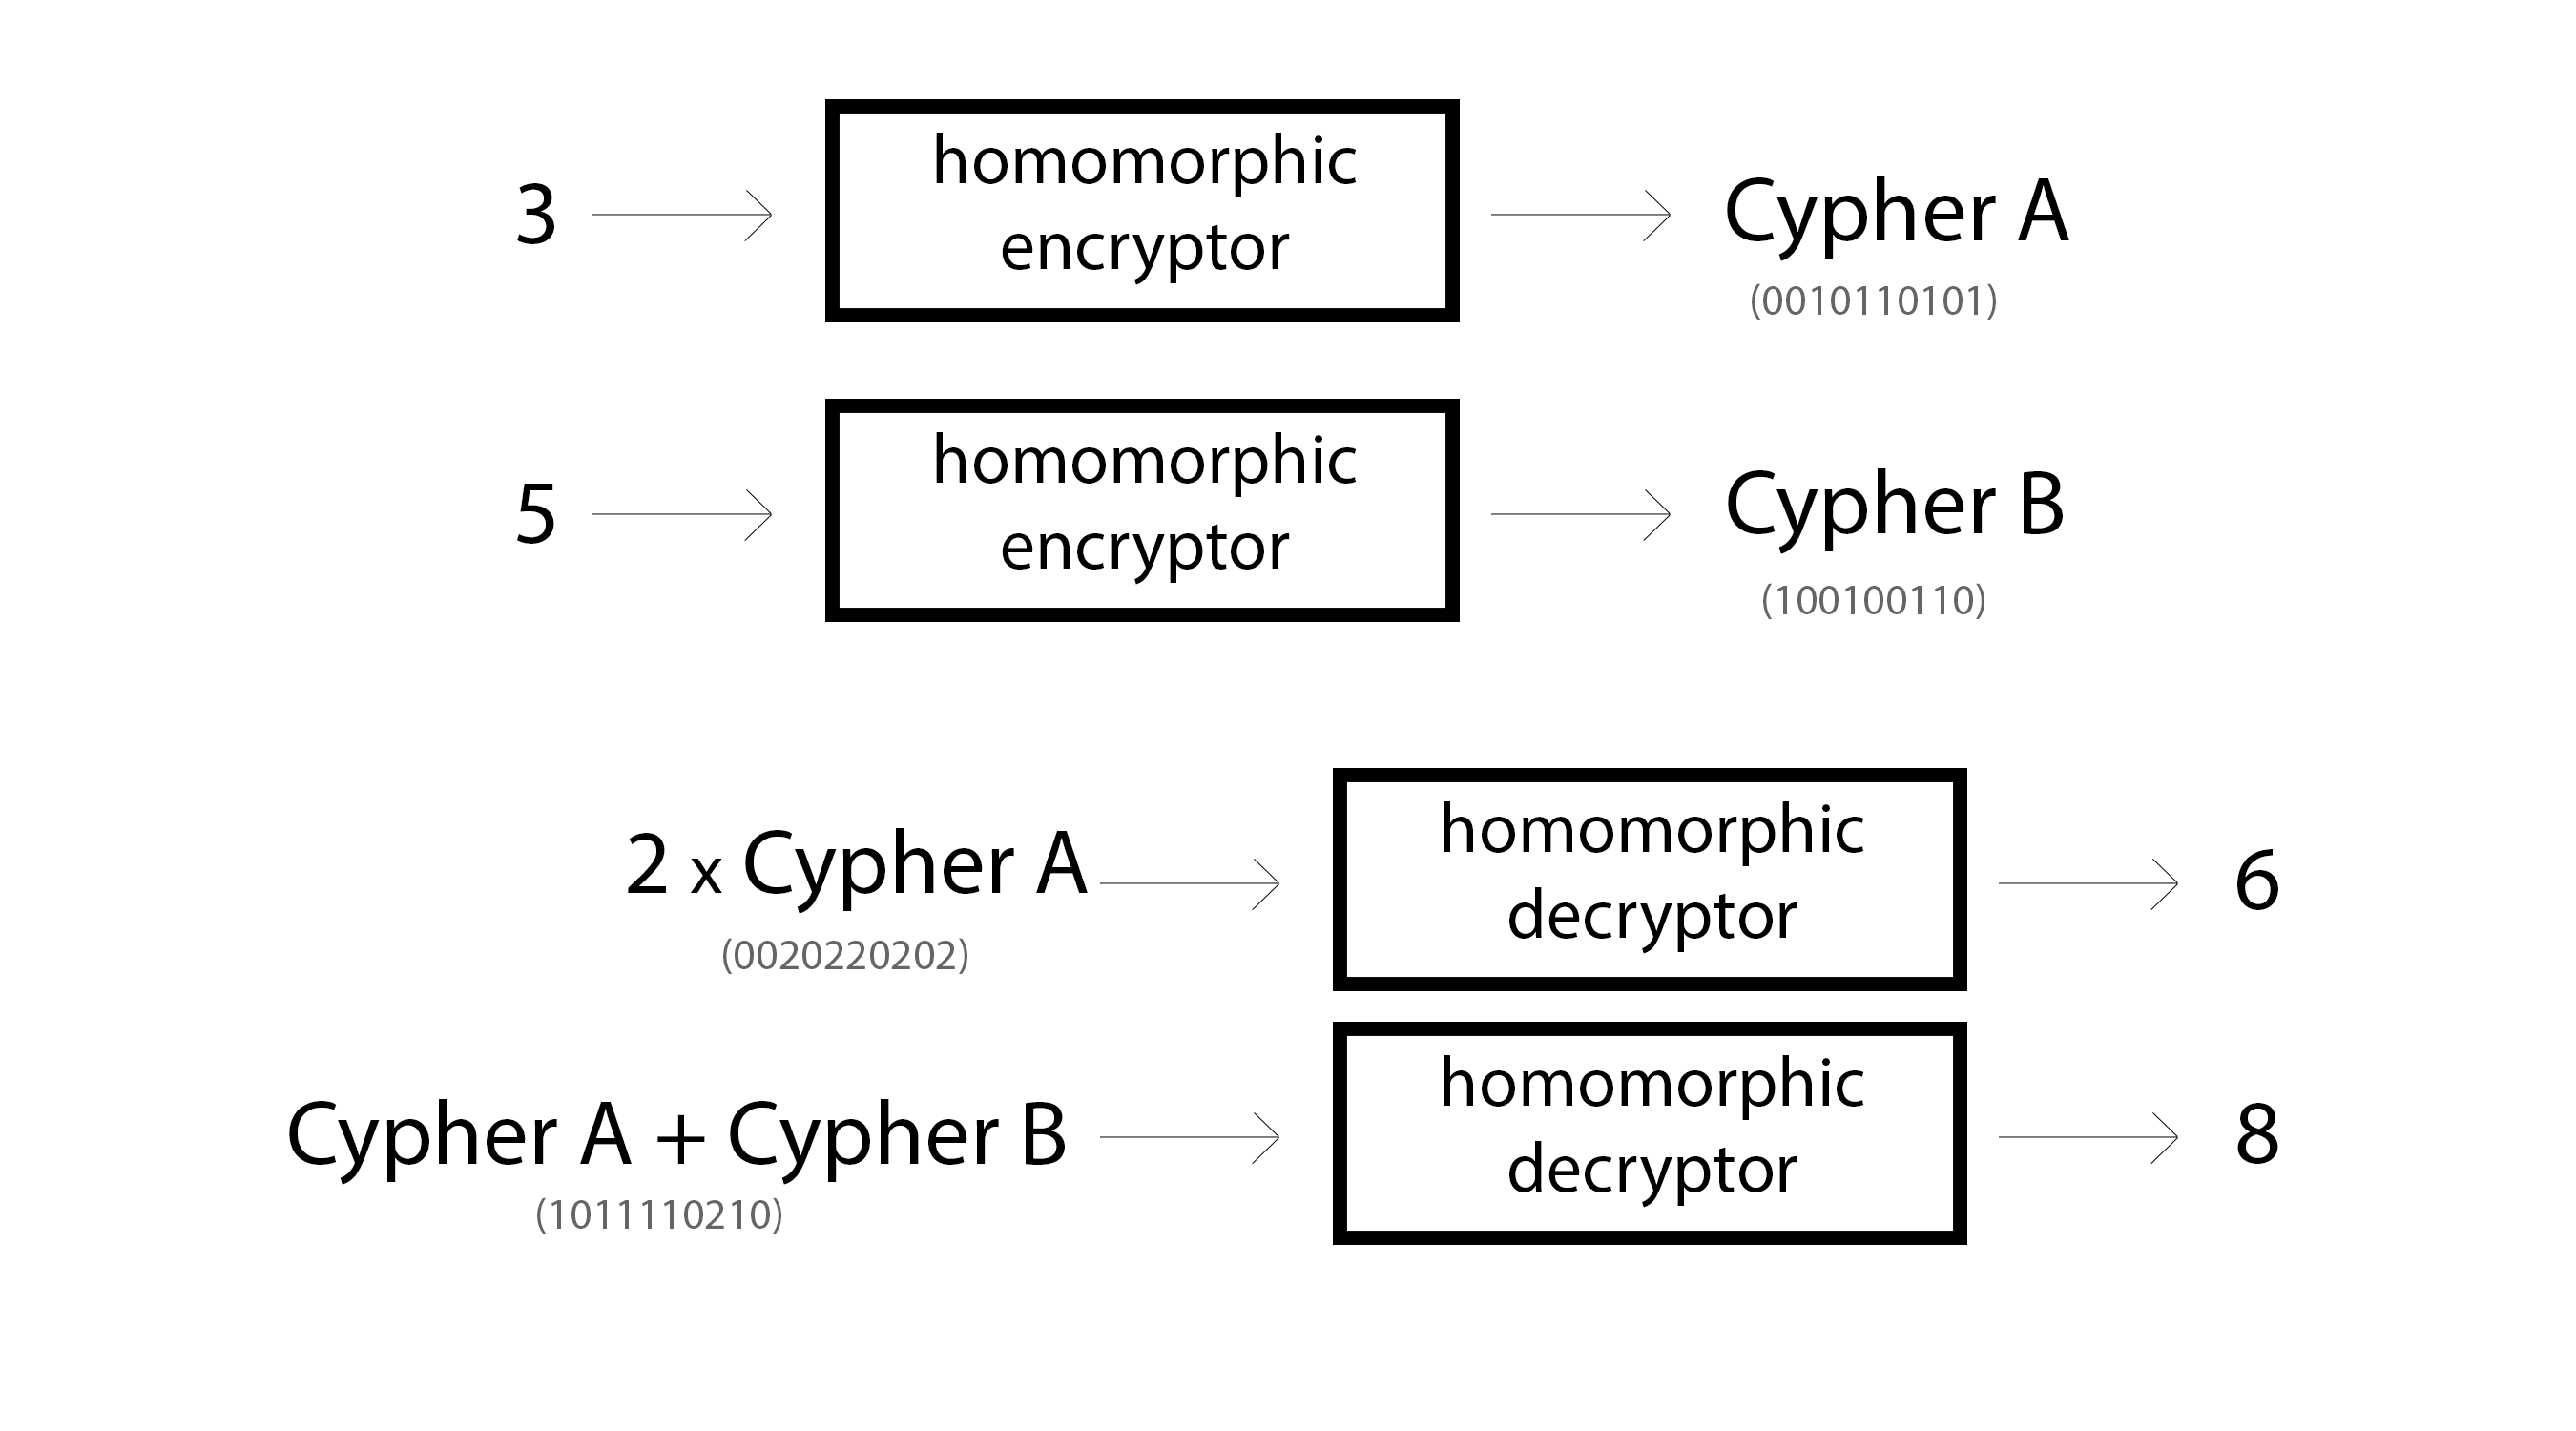
\includegraphics[scale=0.5]{imgs/he.png}
	\caption{\cite{he} Ejemplos de operaciones matemáticas realizadas sobre números encriptados por medio de Homomorphic Encryption.}
\end{figure}


\section{Differential Privacy}
La privacidad diferencial \cite{diffpriv4} no es, en sí misma, una tecnología. Es una propiedad que describe algunos sistemas: una garantía matemática de que no se violará la privacidad uno o mas individuos si sus datos se utilizan para un determinado análisis. Un sistema que es diferencialmente privado permite realizar análisis sobre estos datos sensibles mientras los protege detrás de un velo de incertidumbre. \\
Otra definición \cite{diffpriv3} lo describe una promesa hecha por aquellos individuos o entes que recaban o curan datos, a los due\~nos originales de los mismos. Dicha promesa expresa que la privacidad del dueño original no ser\'a afectada de forma adversa al permitir que sus datos sean usados en alg\'un estudio o an\'alisis, no importa qu\'e otros estudios, sets de datos o fuentes de informaci\'on haya disponibles.

\subsection{Local Differential Privacy}
Con la privacidad local, no hay una parte confiable; cada persona es responsable de agregar ruido a sus propios datos antes de compartirlos. Cada persona es un curador a cargo de su propia base de datos privada. Por lo general, un sistema privado local involucra a una parte no confiable (el agregador) que recopila datos de un gran grupo de personas a la vez.

\subsection{Global Differential Privacy}
Los sistemas privados a globales son generalmente más precisos: todo el análisis se realiza en datos "limpios", y solo se necesita agregar una pequeña cantidad de ruido al final del proceso. Sin embargo, para que funcione la privacidad global, todos los involucrados deben confiar en el curador. \\
La privacidad local es un modelo más conservador y seguro. Bajo la privacidad local, cada dato individual es extremadamente ruidoso y no es muy útil por sí solo. Sin embargo, en números muy grandes, el ruido de los datos se puede filtrar, y los agregadores que recopilan suficientes datos privados locales pueden hacer análisis útiles sobre las tendencias en todo el conjunto de datos.

\begin{figure}[H]
  	\centering
	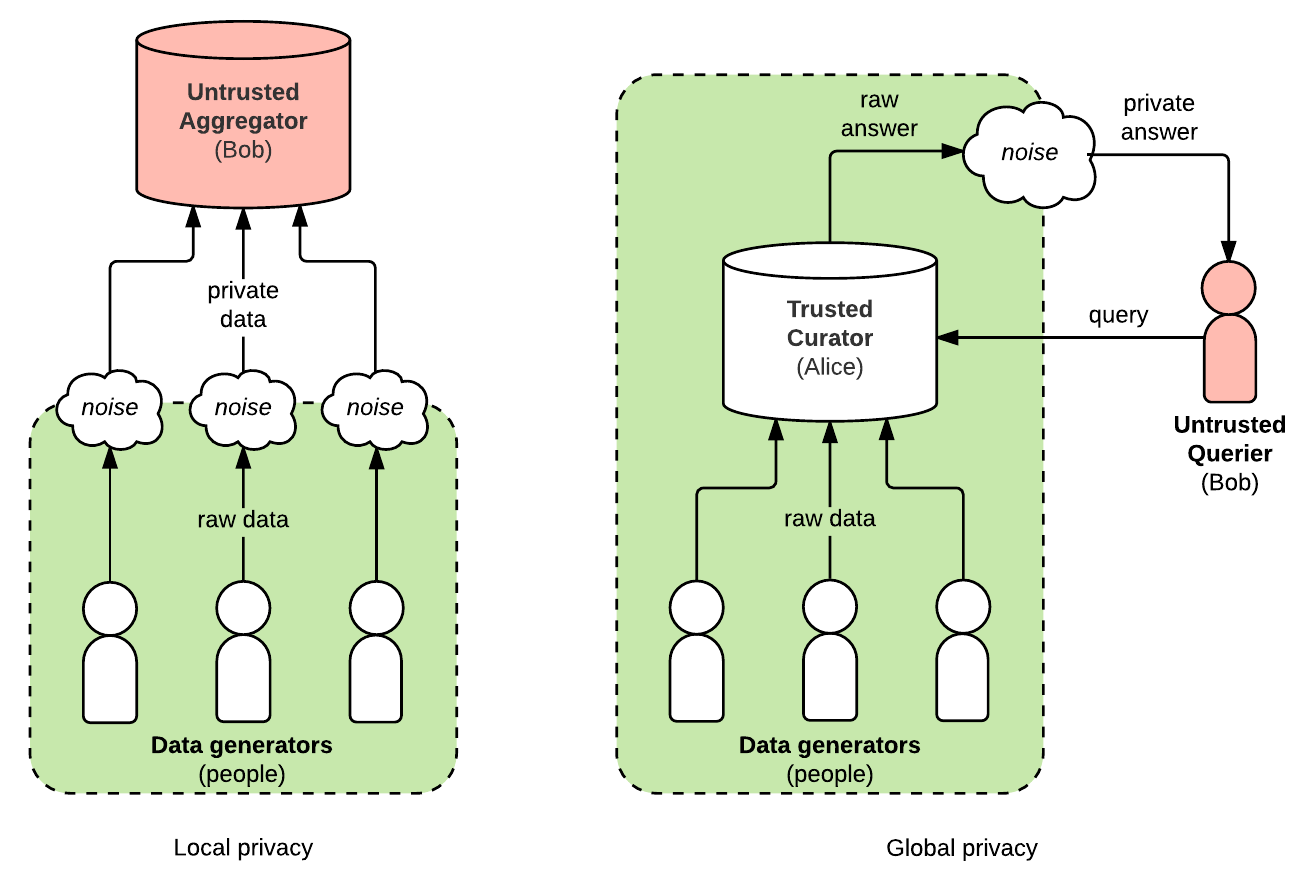
\includegraphics[scale=0.7]{imgs/diff-privacy.png}
	\caption{Local Differential Privacy vs. Global Differential Privacy}
\end{figure}



\section{Trustless}



\section{Federated Learning}
El aprendizaje federado es un método de aprendizaje automático en el que el objetivo es entrenar a un modelo centralizado de alta calidad con datos de entrenamiento distribuidos entre un gran número de clientes, cada uno con conexiones de red poco confiables y relativamente lentas. Los algoritmos de aprendizaje para esta configuración funcionan de la siguiente manera: en cada iteración, cada cliente calcula de forma independiente una actualización del modelo actual en función de sus datos locales y comunica esta actualización a un servidor central, donde las actualizaciones enviadas por los clientes se agregan para calcular una nueva versión global del modelo.

\begin{figure}[H]
  	\centering
	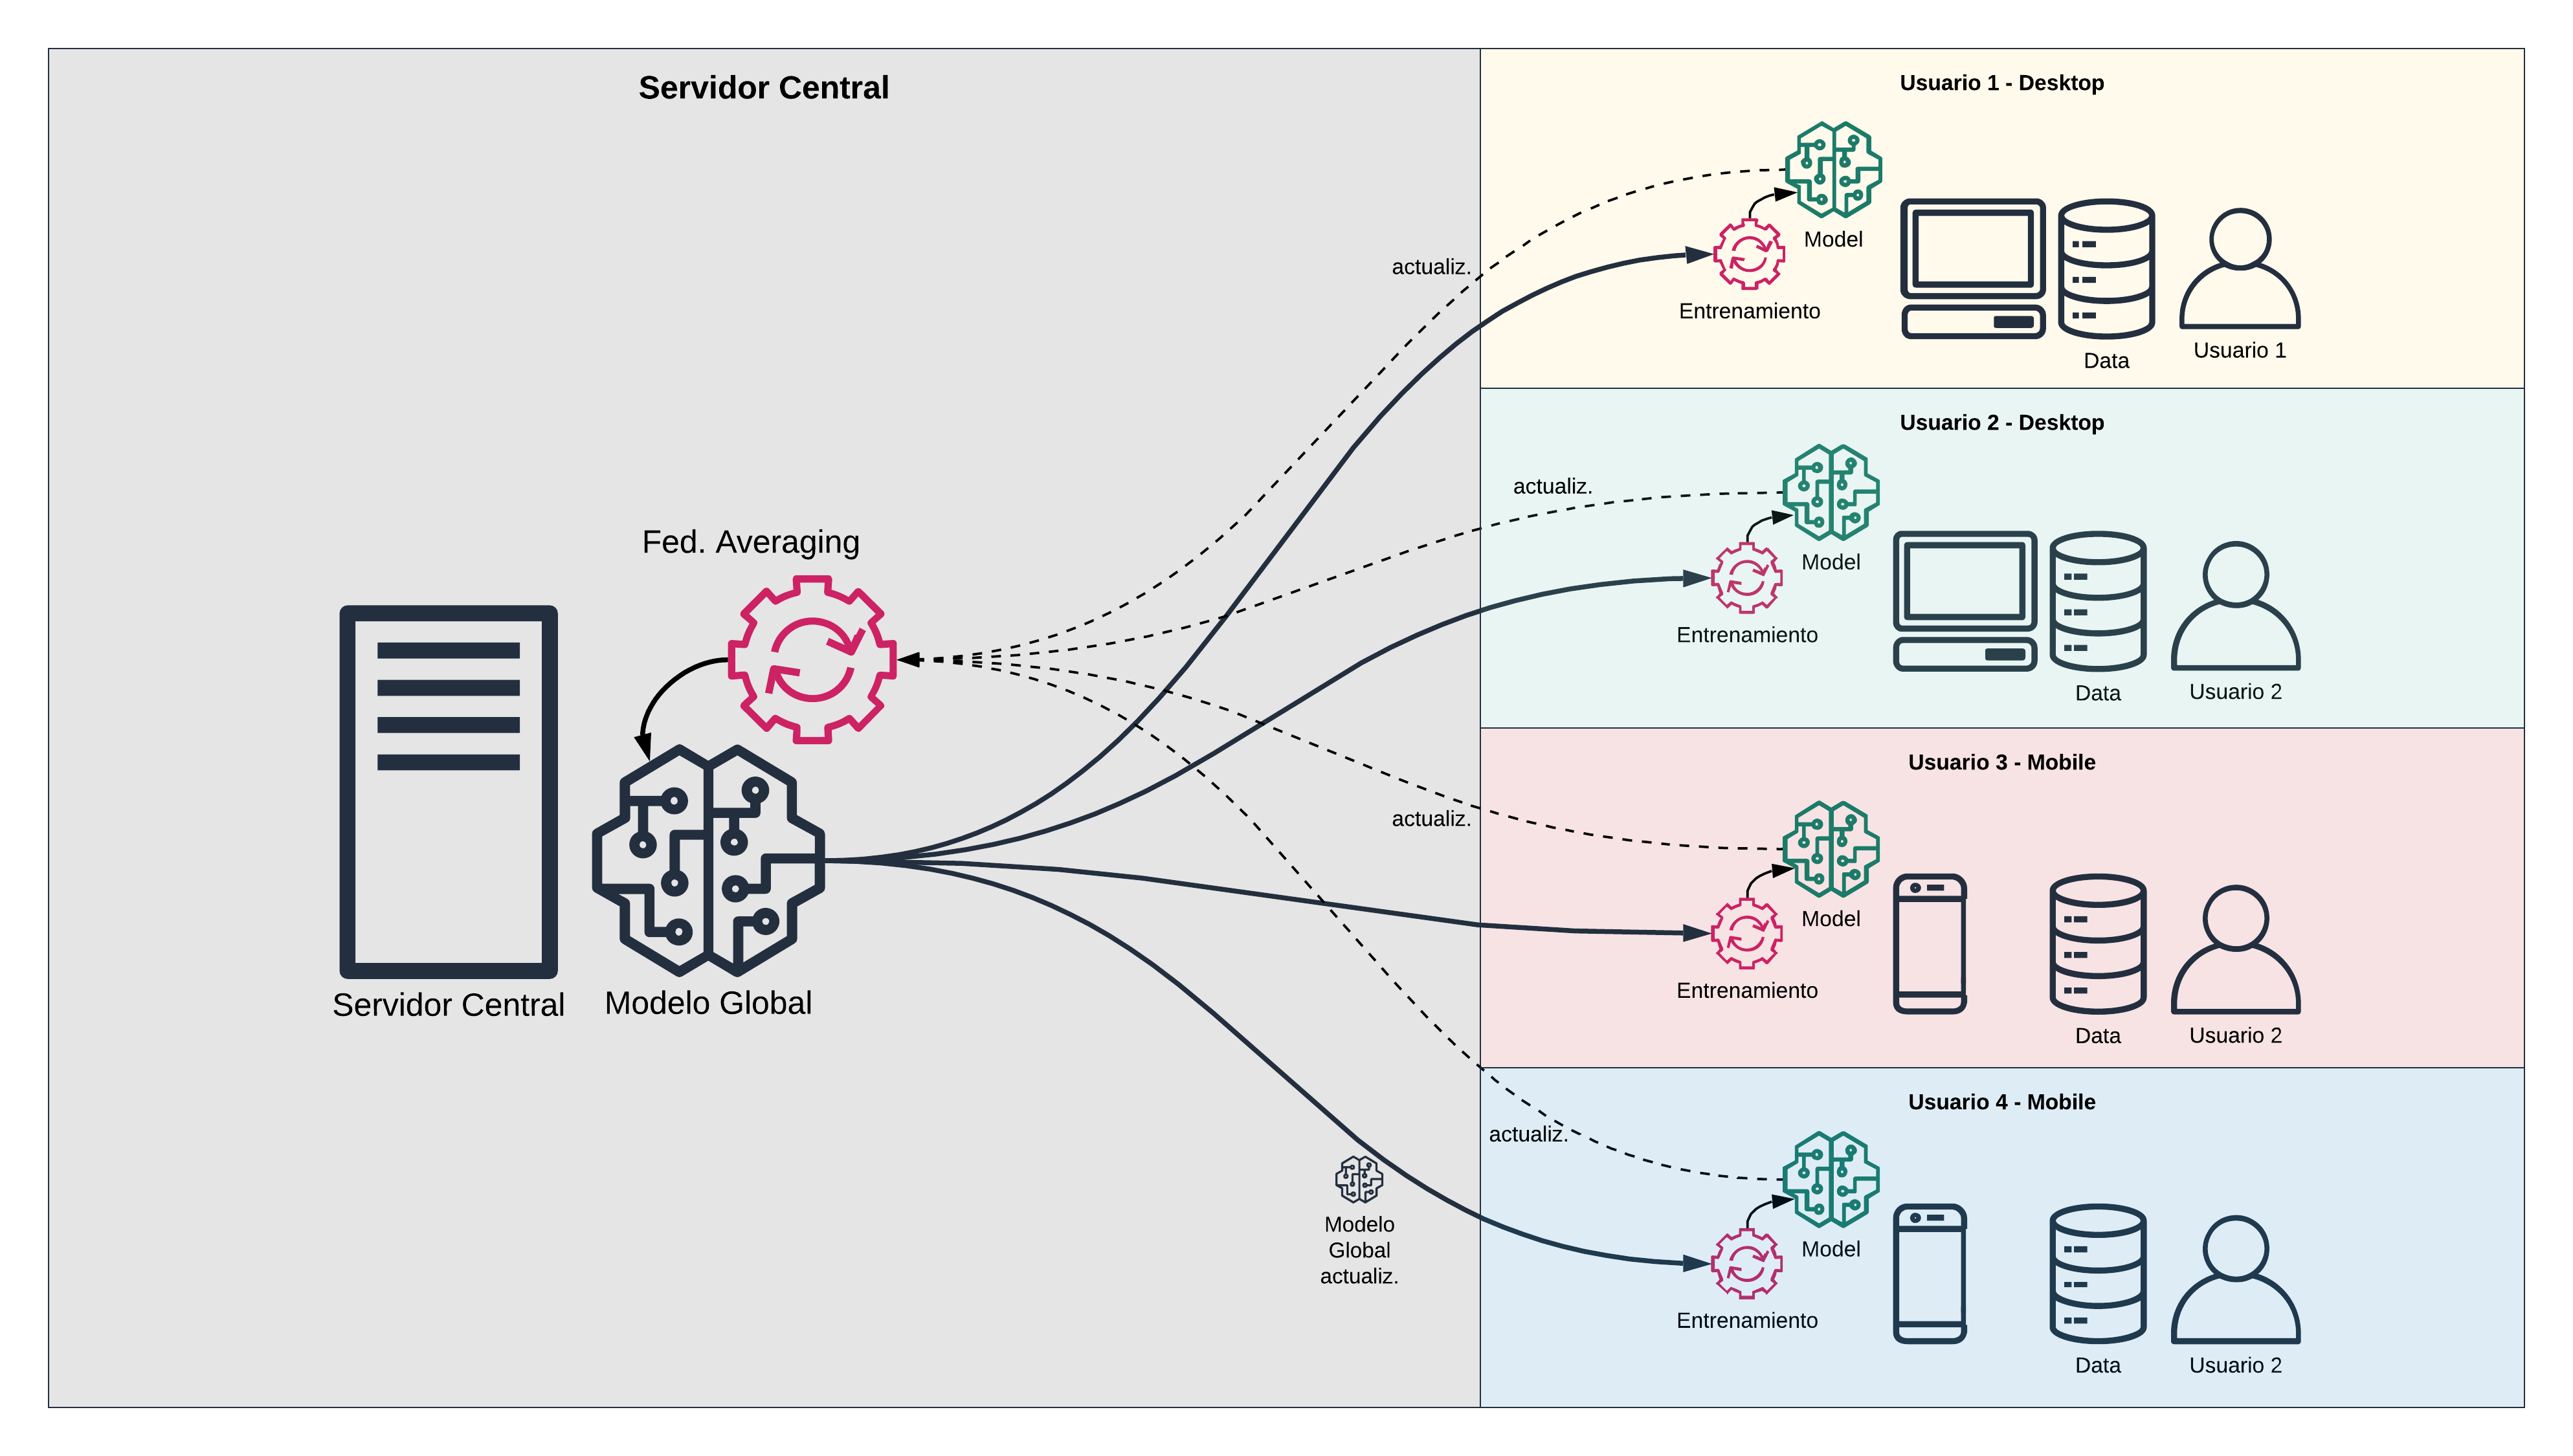
\includegraphics[scale=0.42]{imgs/fl_flow.png}
	\caption{Esquema de entrenamiento de un modelo usando Federated Learning.}
\end{figure}


\section{Módulos}

\subsection*{Interacción entre modulos}
A continuación mostramos un diagrama del sistema describiendo las interacciones entre los diferentes módulos. \\

\begin{figure}[H]
  	\centering
	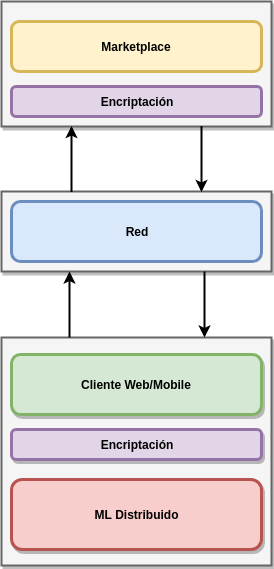
\includegraphics[scale=0.5]{imgs/modules-diagram.png}
	\caption{Interacciones de los módulos del sistema}
\end{figure}

\subsection*{Módulo de Machine Learning distribuido}
Este módulo tendrá como responsabilidad realizar entrenamientos de modelos de Machine Learning siguiendo el esquema de Federated Learning. Tendrá una interfaz lo suficientemente genérica como para poder usarse con un servidor central o en una red de nodos descentralizados (como se pretende hacer con la red de Ethereum).

\subsection*{Módulo de encriptac\'ion}
La responsabilidad de este módulo será la encriptación y desencriptación de los modelos que se transfieran en la red para su entrenamiento. \\
Para evitar el envío de datos por la red, y así preservar la privacidad, el esquema de Federated Learning establece que se envíen los modelos a los clientes que los entrenarán.
Dichos modelos deben estar encriptados, ya que de otra forma cualquier participante malicioso de la red podría robarlo. \\
Para poder operar sobre un modelo encriptado existen técnicas tales como Homomorphic Encryption. \\
El módulo deberá minimizar el riesgo de violación de la privacidad tanto del usuario que entrena el modelo con sus datos, como del usuario que desea obtener un modelo entrenado (sin que nadie se lo robe en el proceso), para esto se explorarán técnicas de  Secure Multi party computation y Differential Privacy \cite{diffpriv1} \cite{diffpriv2}.

\subsection*{La red}
La red constará de uno o mas smart contracts desplegados en la red de Ethereum que estarán integrados con IPFS como método de almacenamiento descentralizado.
La red proveerá medios para recompensar a los participantes de la misma, tales como pueden ser los usuarios que entrenan los modelos, según el nivel de su aporte a la calidad de las predicciones del modelo.

\subsection*{Interfaz web del marketplace}
El sistema debe tener una interfaz web que permita que usuarios puedan construir un modelo de machine learning que use determinado tipo de datos y enviarlo para su entrenamiento a los diferentes nodos de la red que cumplan con las características pedidas por el usuario dueño del modelo.

\subsection*{Cliente web/mobile}
Este cliente deberá permitir que los usuarios decidan cuales de sus datos quieren que sean usados para entrenar modelos de machine learning.

\newpage

\chapter{Implementación}

\section{Participantes}

\subsection*{DeltaML: Interacción entre participantes}
En la figura \ref{fig:interact} se observa se observa un diagrama del sistema y describimos cada una de las interacciones entre los diferentes participantes.

\begin{figure}[h!]
  	\centering
	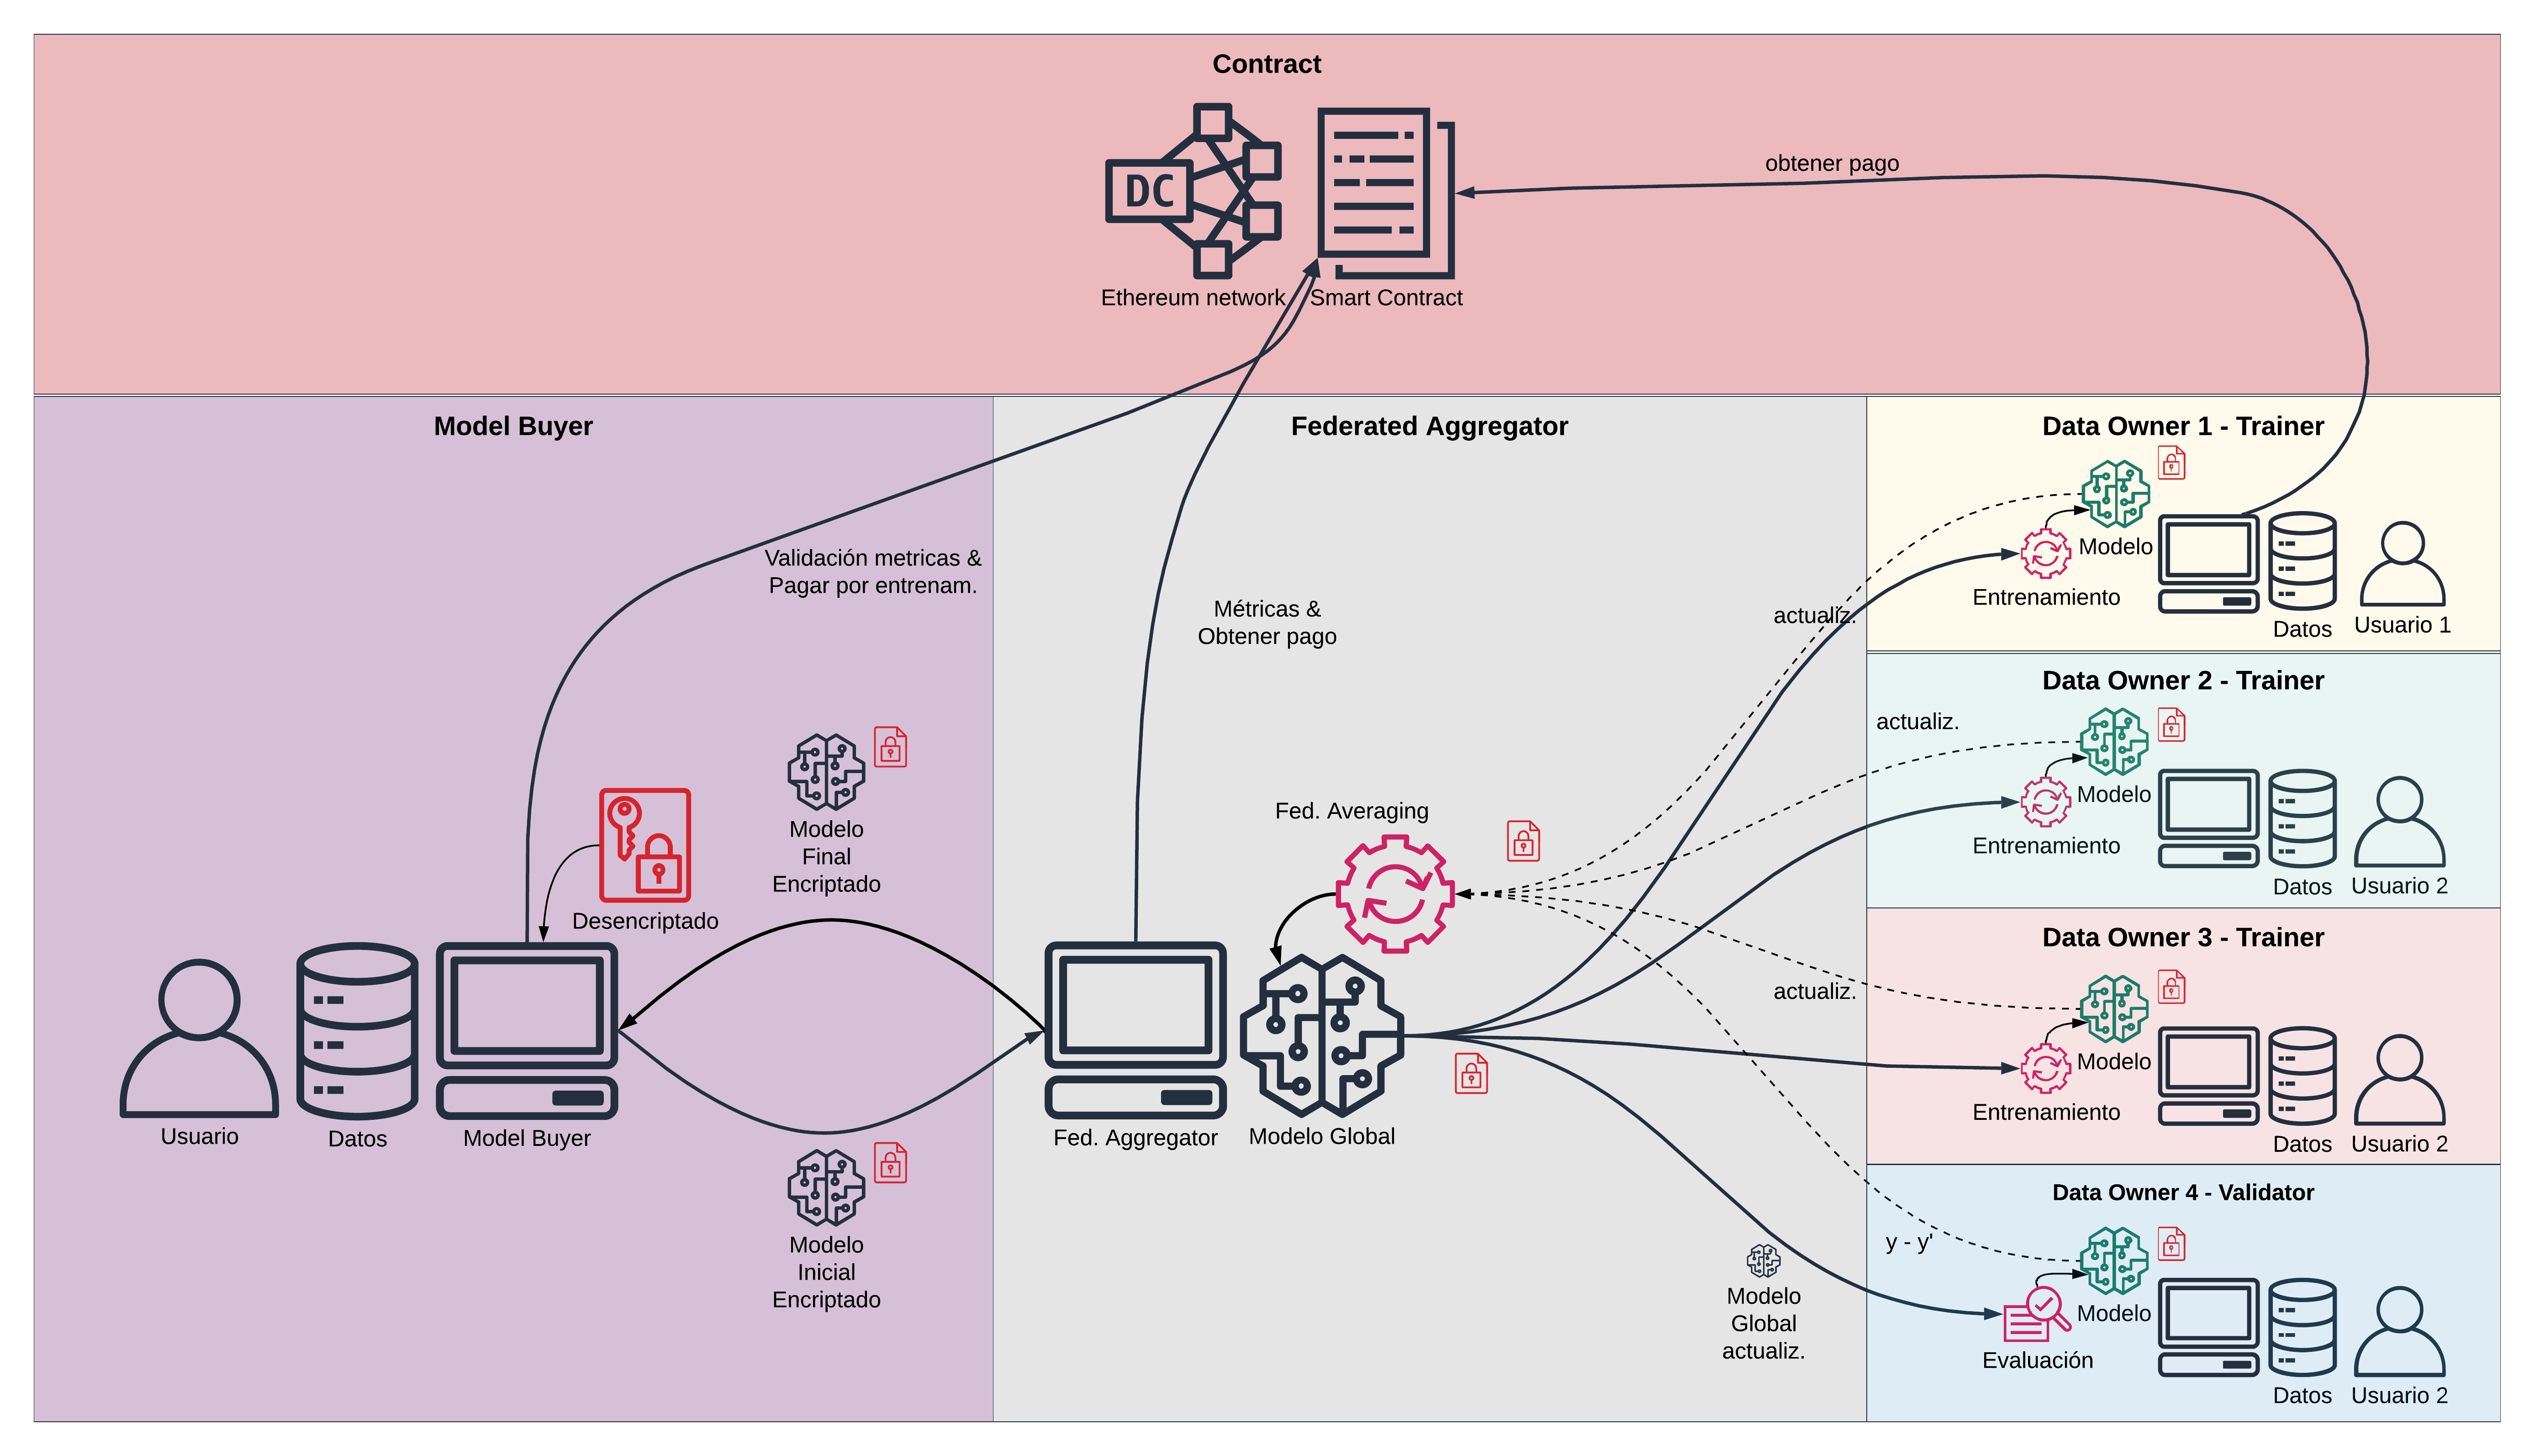
\includegraphics[scale=0.072]{imgs/deltaml_flow.png}
	\caption{Interacciones de los módulos del sistema}
	\label{fig:interact}
\end{figure}


\subsection*{Data Owner}
\justify
El Data Owner es aquel que ejecuta en su computador el cliente web por medio del cual puede decidir en qué solicitudes de entrenamiento participar. Tiene en su poder uno o mas datasets. \\
En su rol de de Data Owner publica al smart contract las caracteristicas de los datasets que posee (cantidad de registros, columnas, tipo de los datos de cada columna, cantidad de nulos por columna, etc) y recompensa monetaria mínima que está dispuesto a percibir por el entrenamiento de cada dataset.

\subsubsection*{Capacidades}
\begin{itemize}
\item Elige participar en el entrenamiento de un modelo.
\item Aporta sus datos para, de manera local y sin poder ver el modelo:
\item Entrenar el modelo solicitado por el Model Buyer.
\item Calcular diferencia entre predicciones del modelo y lo esperado.
\end{itemize}

\subsubsection*{Limitaciones}
No puede:
\begin{itemize}
\item Ver los parámetros del modelo en entrenamiento, trabaja con el modelo encriptado.
\item Alterar el cálculo de las métricas de calidad o su contribución para ganar más dinero por el entrenamiento. 
\end{itemize}

\subsubsection*{Roles}
\begin{itemize}
\item \textbf{Trainer:} Usa sus datos privados y su poder de cómputo para entrenar modelos.
\item \textbf{Validator:} Usa sus datos privados y su poder de cómputo para  calcular diferencias entre lo esperado y las predicciones.
\end{itemize}

Los Data Owners se dividen en Trainers y Validators en proporciones de 70\% y 30\% respectivamente tal como se haría con un dataset para su entrenamiento y evaluación. Queda para futuros desarrollos hacer esta división emulando un K-Fold Cross-validation.


\subsection*{Model Buyer}
\justify
El Model Buyer interactua con el sistema por medio del marketplace, publicando una solicitud de entrenamiento para un cierto modelo con ciertas caracteristicas.
Al crear la solicitud envía un modelo inicial encriptado con Homomorphic Encryption al Federated Aggregator junto con  las carácteristicas que debe cumplir el dataset para entrenar el modelo. 
Al mismo tiempo, inicializa en un smart contract desplegado en la red Ethereum, la transacción del correspondiente al entrenamiento del modelo y envía el monto que destina al proceso de mejorar el modelo inicial, las metricas de calidad del modelo inicial y los participantes involucrados.

\subsubsection*{Capacidades}
\begin{itemize}
\item Solicita el entrenamiento de un modelo.
\item Paga por el modelo entrenado.
\item Desencripta el modelo una vez entrenado.
\item Valida métricas de calidad del modelo.
\end{itemize}

\subsubsection*{Limitaciones}
No puede:
\begin{itemize}
\item Ni ver ni robar los datos con los que se entrenan los modelos.
\item Alterar las métricas de calidad del modelo.
\item Realizar fraude en el pago por el modelo.
\end{itemize}



\subsection*{Federated Aggregator}
Este participante del sistema verifica periodicamente la existencia de nuevas solicitudes de entrenamiento de modelos consultando al smart contract. De encontrar una nueva solicitud, obtiene del smart contract el hash que corresponde al directorio donde se almacenan los recursos referentes a esta solicitud en IPFS, y comienza a verificar si hay nuevas mejoras publicadas por los Trainers. De existir nuevas mejoras, el Federated Aggregator realiza un promedio de las mejoras al modelo y el modelo inicial, luego calcula la métrica de calidad del modelo nuevamente y la envia al smart contract.

\subsubsection*{Capacidades}
\begin{itemize}
\item Asigna roles a los Data Owners que participan en un entrenamiento.
\item Agrega de manera segura las actualiz. al modelo provenientes de cada Data Owner.
\item Envía el modelo actualiz. encriptado a los Data Owners para que continúen el entrenamiento.
\item Calcula las métricas de calidad del modelo.
\end{itemize}

\subsubsection*{Limitaciones}
No puede:
\begin{itemize}
\item Robar el modelo en entrenamiento, está encriptado.
\item Alterar el cálculo de las métricas de calidad ni las contribuciones de cada Data Owner (las valida el Model Buyer).
\end{itemize}


\subsection*{Contract}
El smart contract es el encargado de regular el mercado, recibe solicitudes provenientes del Model Buyer y las vincula con los Data Owners que las acepten y al modelo en entrenamiento. Al mismo tiempo, permite al Federated Aggregator guardar métricas métricas de calidad del modelo y que sean validadas por el Model Buyer.
Se define aquí tambien, la recompensa mínima que recibirán todos los participantes del entrenamiento (monto fijo) y el monto variable de acuerdo a la contribución a la mejora de la calidad del modelo. \\
El carácter descentralizado del smart contract permite que los cálculos y pagos se realicen sin necesitar de una tercera parte en la que confiar para esta parte del proceso.


\subsubsection*{Capacidades}
\begin{itemize}
\item Restringe el acceso a sus funcionalidades según el rol del participante.
\item Calcula contribuciones de cada Data Owner.
\item Paga a cada participante por su trabajo.
\item Devuelve dinero al Model Buyer si tuviera que hacerlo.
\item Valida métricas de calidad del modelo.
\end{itemize}

\subsubsection*{Limitaciones}
No puede:
\begin{itemize}
\item Robar el modelo en entrenamiento (no tiene visión del mismo).
\item Alterar el cálculo de las métricas de calidad.
\item Alterar el cálculo de las contribuciones.
\end{itemize}

\section{Protocolos}

\subsection*{Obtención de recursos para entrenamiento}
\begin{figure}[H]
  	\centering
	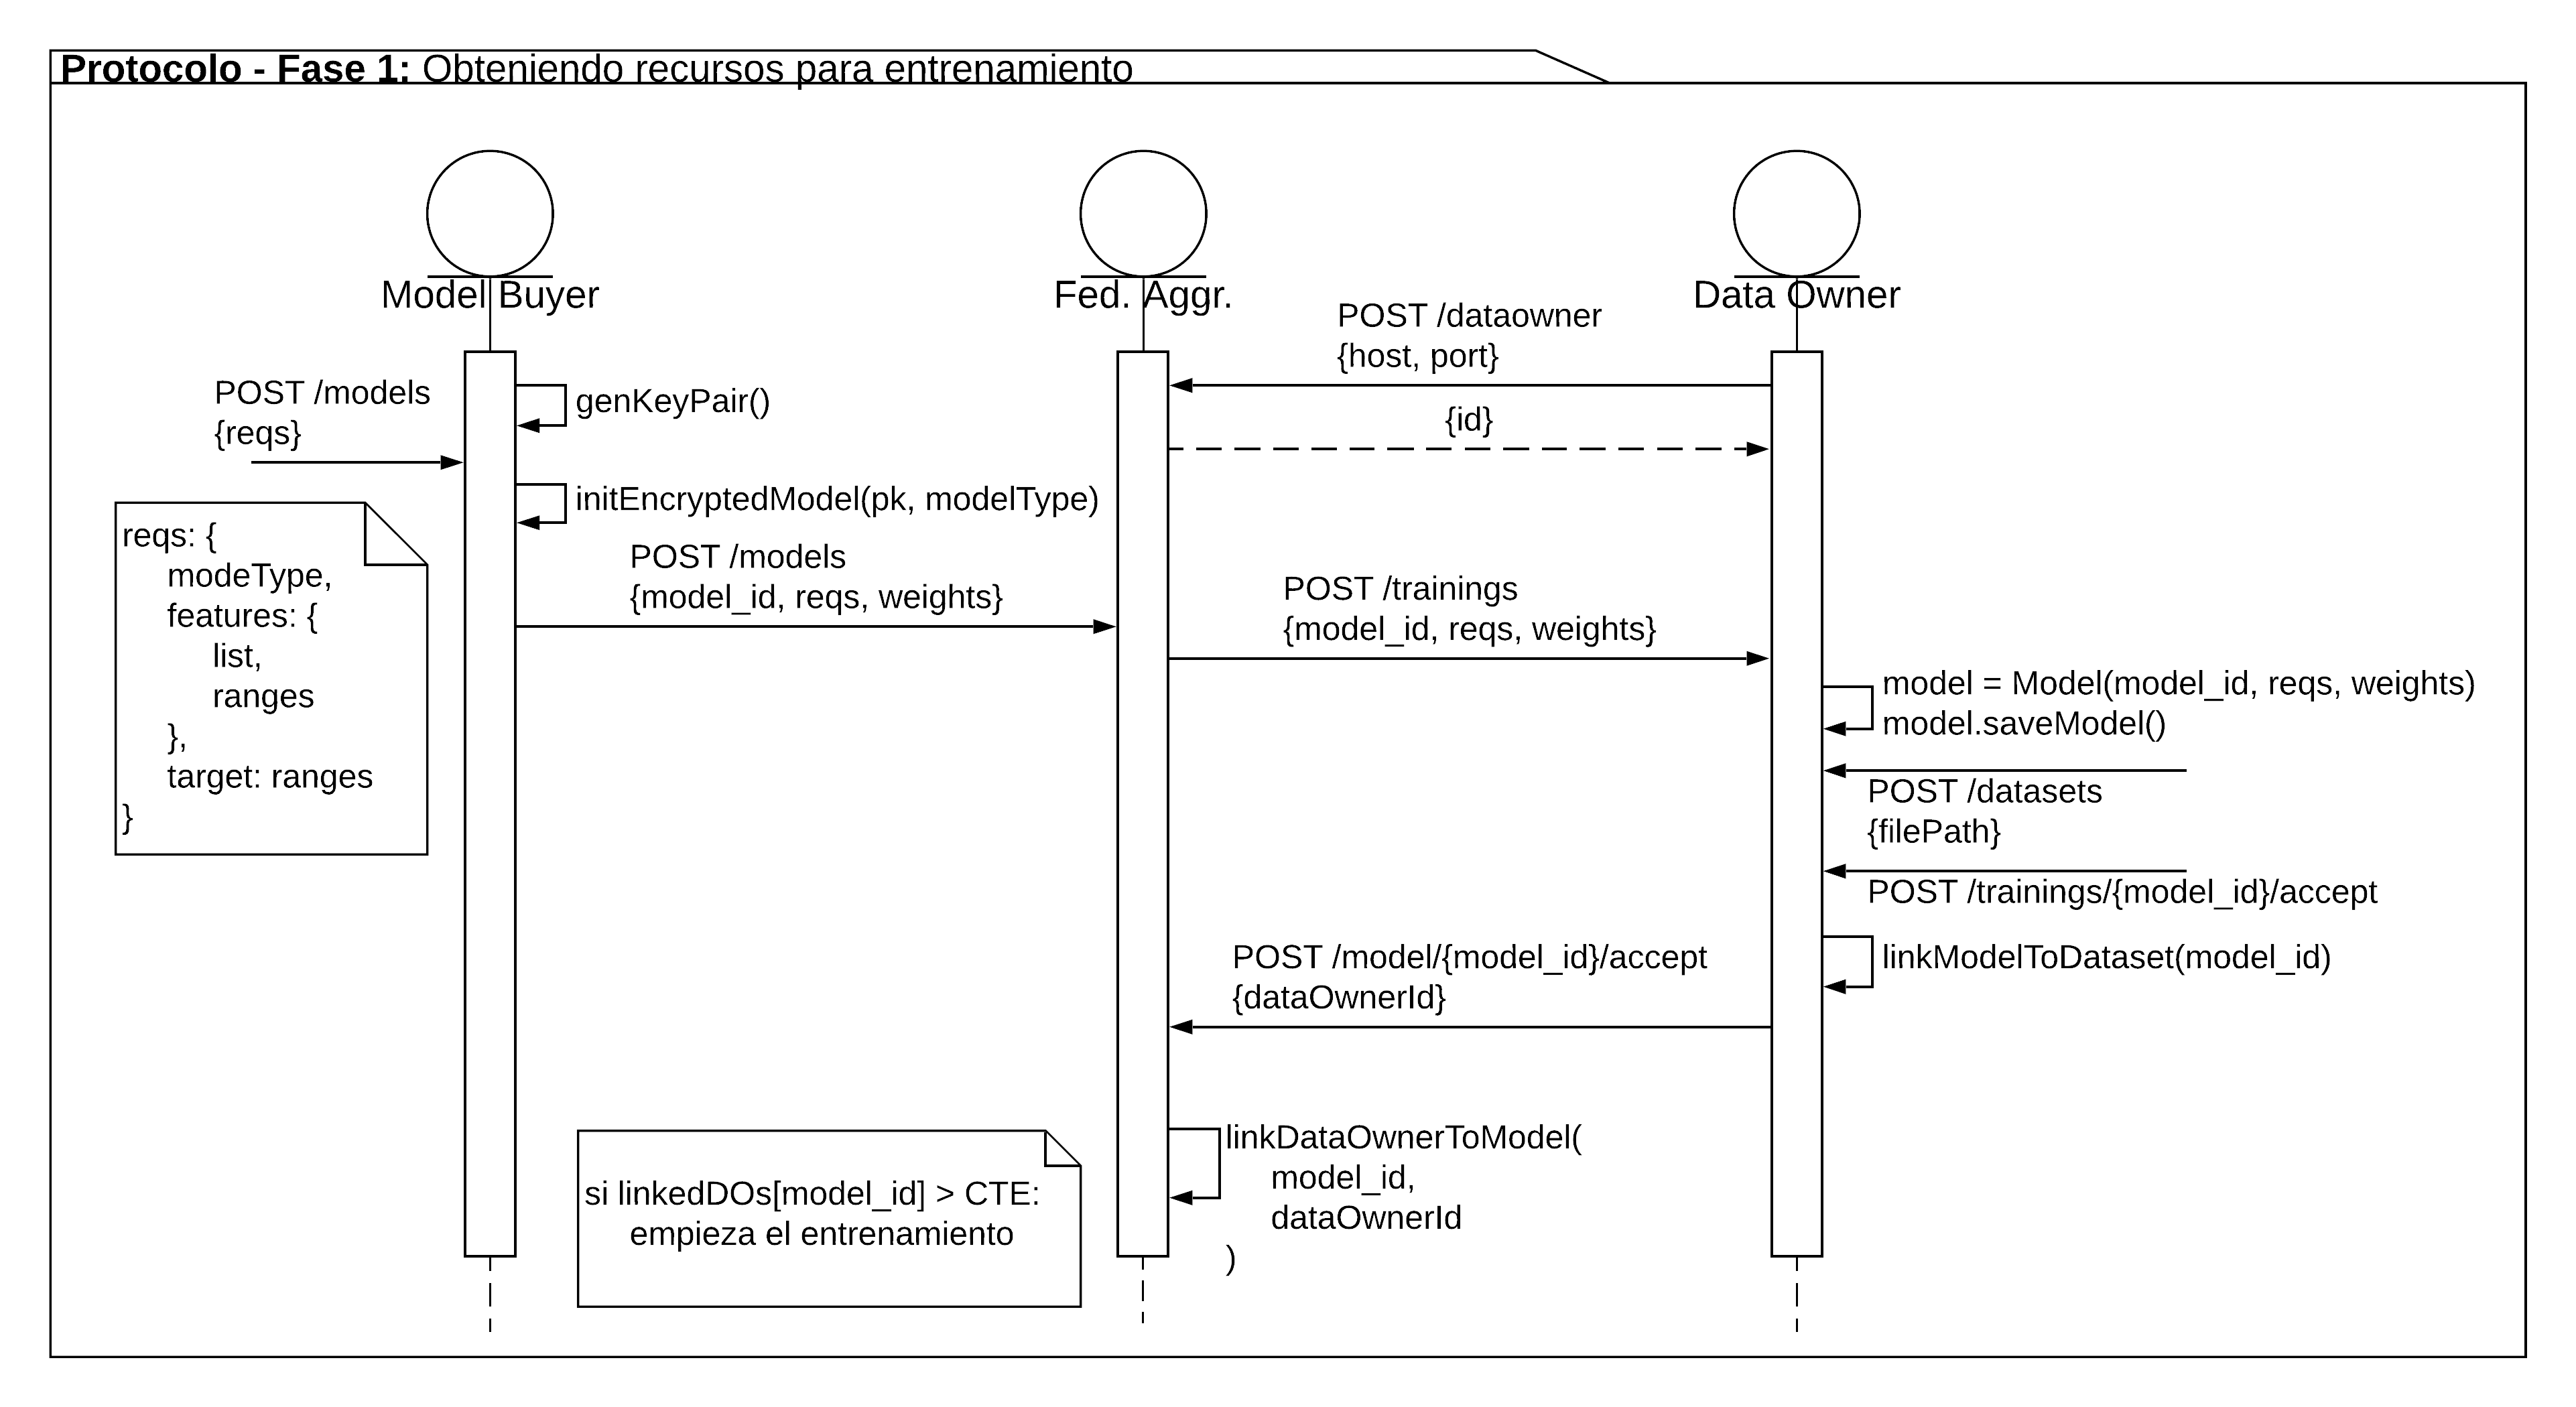
\includegraphics[scale=0.1]{imgs/flujo_fase1.png}
	\caption{Esquema de entrenamiento de un modelo usando Federated Learning.}
\end{figure}

\subsection*{Entrenamiento del modelo encriptado}
\begin{figure}[H]
  	\centering
	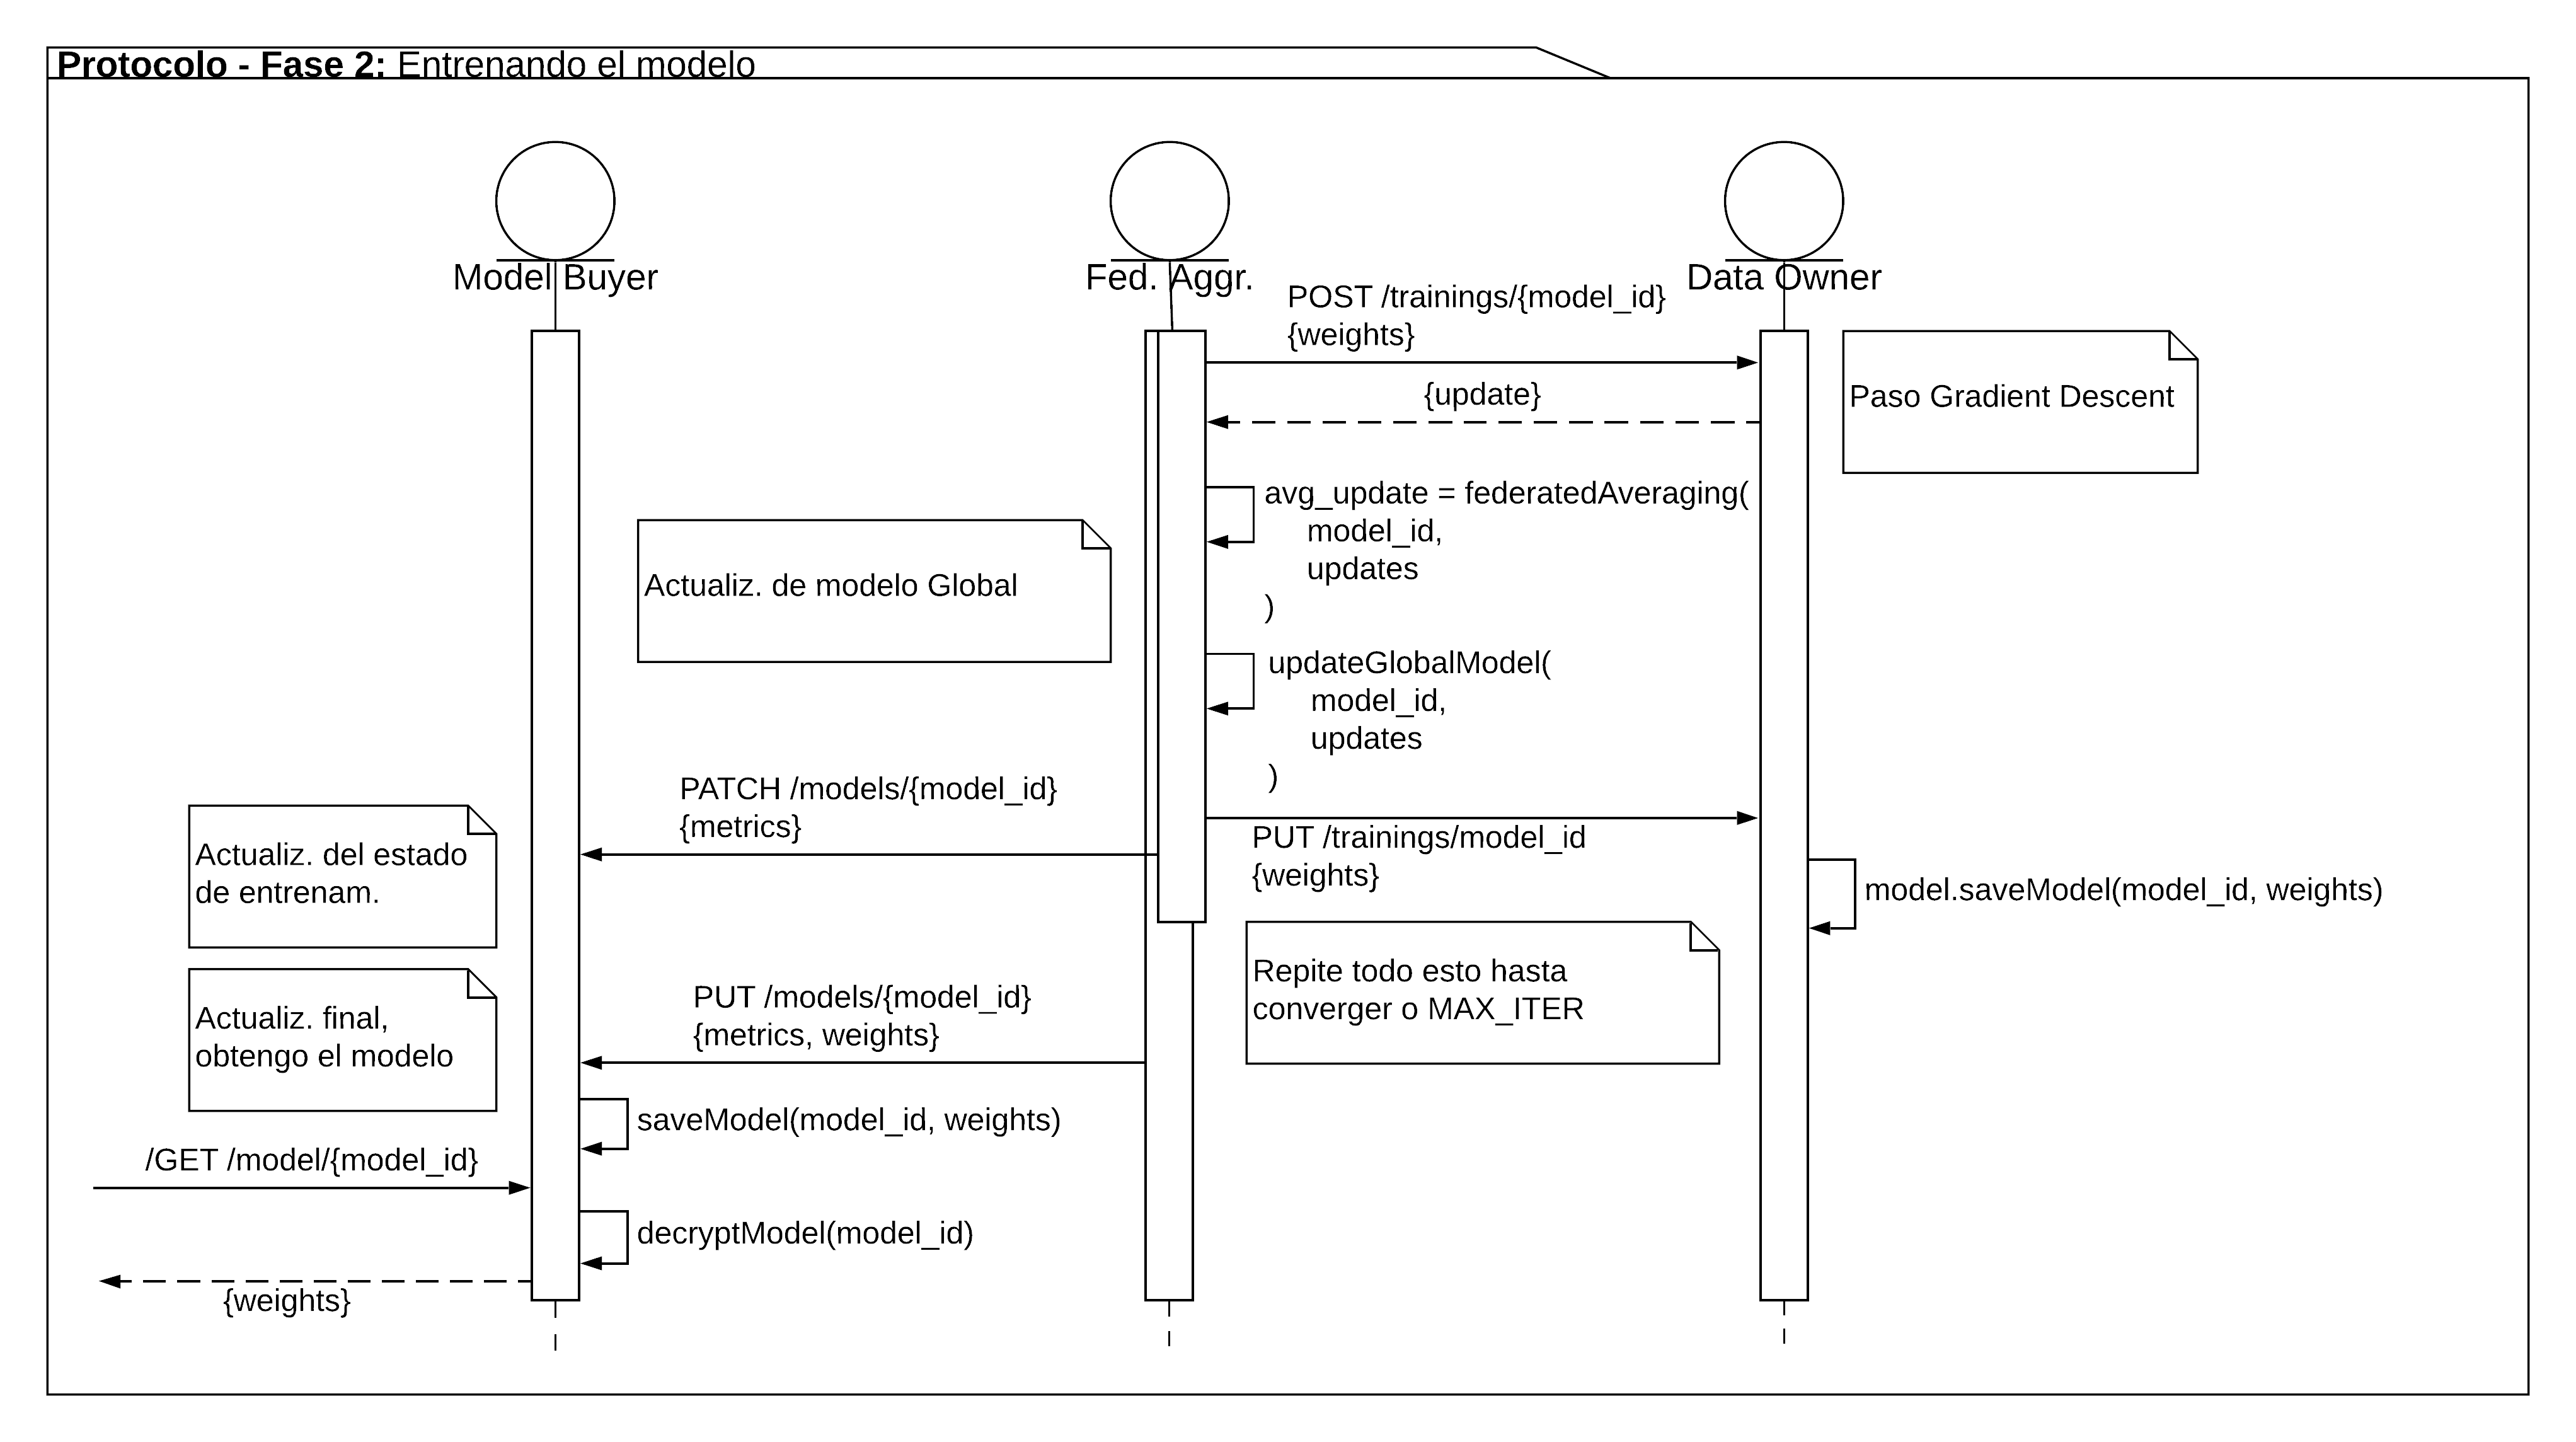
\includegraphics[scale=0.1]{imgs/flujo_fase2.png}
	\caption{Esquema de entrenamiento de un modelo usando Federated Learning.}
\end{figure}

\subsection*{Calculo de métricas seguro}
\begin{figure}[H]
  	\centering
	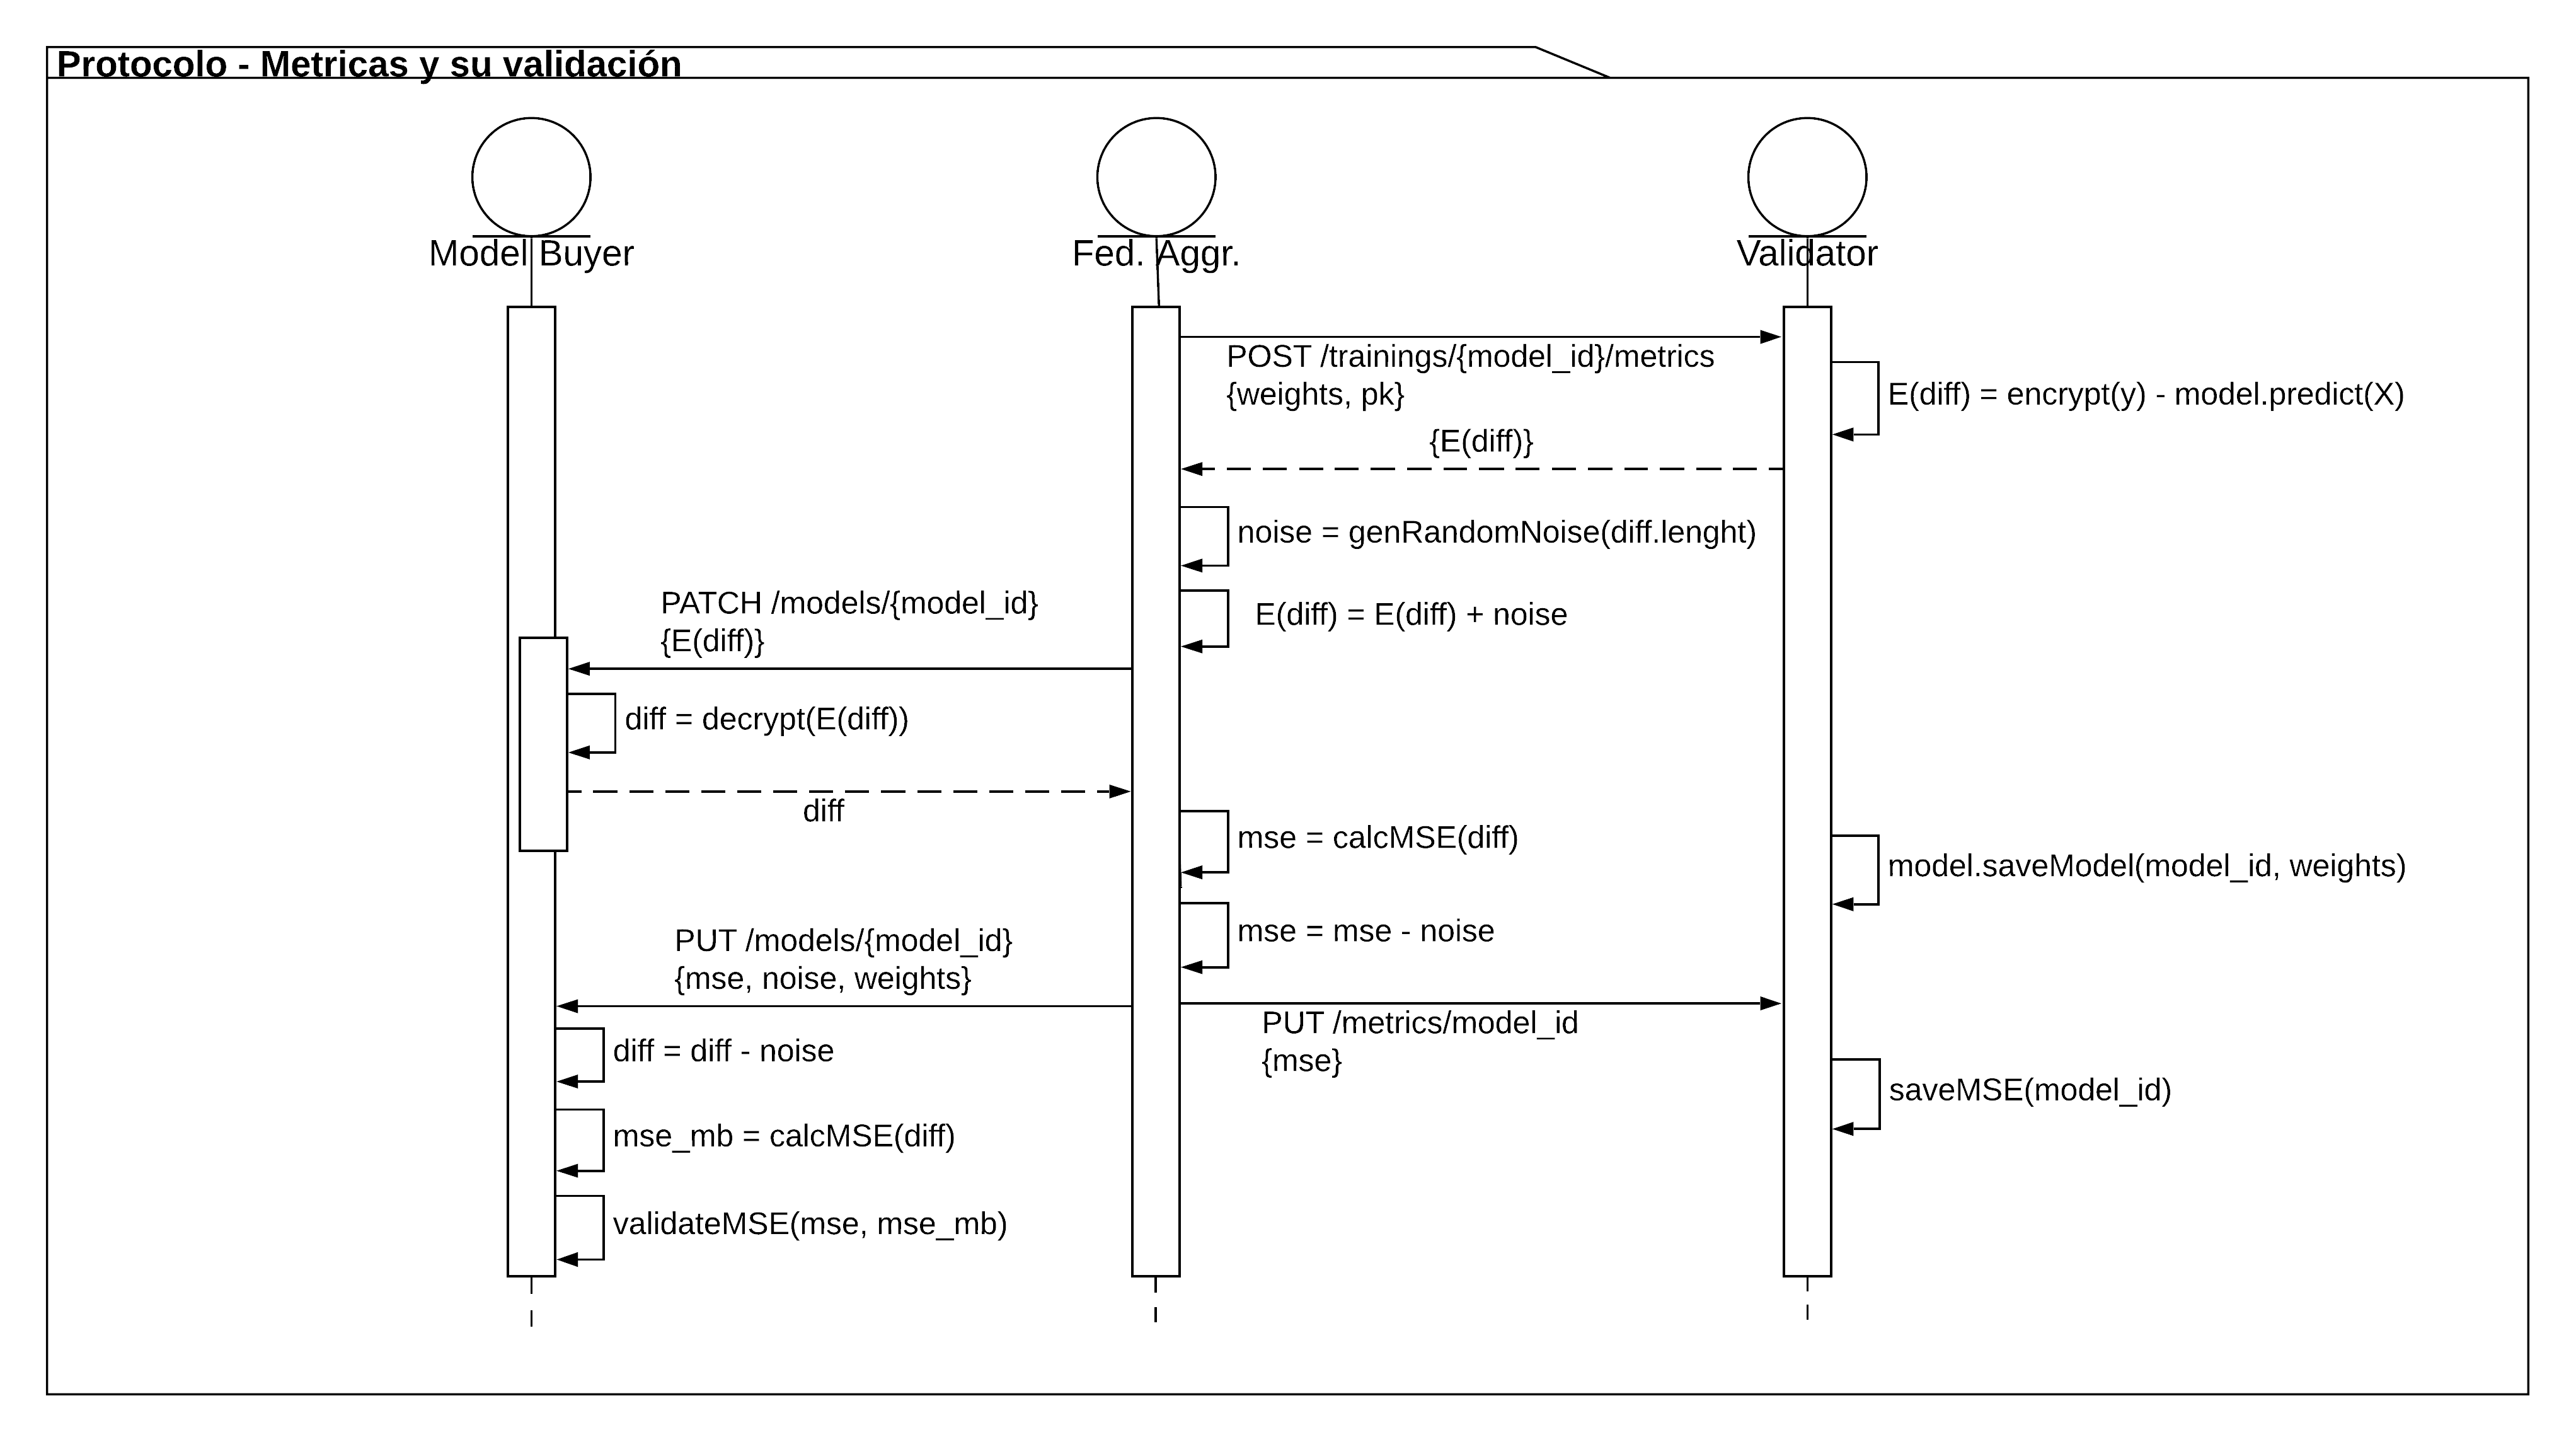
\includegraphics[scale=0.1]{imgs/flujo_valid.png}
	\caption{Esquema de entrenamiento de un modelo usando Federated Learning.}
\end{figure}


%----------------------------------------------------------------------------------------
%	BIBLIOGRAPHY
%----------------------------------------------------------------------------------------

\printbibliography[heading=bibnumbered, title=Referencias]

%----------------------------------------------------------------------------------------
%	GLOSARY
%----------------------------------------------------------------------------------------

\chapter{Glosario}
\begin{itemize}
\item \textbf{Machine Learning}: (en castellano Aprendizaje Automático) es la rama del área de la inteligencia artificial centrada en el estudio y construcción de sistemas capaces de aprender de los datos, identificar patrones y realizar decisiones con mínima intervención humana. 
\item \textbf{Deep Learning}: (o Aprendizaje Profundo) es un subconjunto del área de Machine Learning que intenta generar modelos que constan de arquitecturas compuestas de transformaciones no lineales múltiples. Se utilizan, en general, para resolver problemas de gran complejidad computacional por medio de aproximaciones logradas a través del entrenamiento de un modelo con las caracteristicas antes nombradas a partir de una cantidad enorme de datos.
\item \textbf{Blockchain}: o DLT (Descentralized Ledger Technology), es una tecnología que consta de un registro contable distribuido en una red de nodos. Las características principales de Blockchain son: inmutabilidad de la historia de las transacciones realizadas, resistencia a fraudes utilizando algoritmos de consenso entre los nodos de la red, transparencia (todos los nodos pueden ver el historial de transacciones), resistente a ataques (mediante la descentralización de los datos y el poder de computo combinado de todos los nodos participantes), y pseudo-anonimidad de los participantes de la red (se identifican con una clave que lleva el nombre de wallet, pero a  priori no hay forma de relacionar dicha wallet con su dueño).
\item \textbf{Smart Contract}: aplicaciones que se ejecutan sobre la red de nodos de una blockchain exactamente como fueron programadas sin ninguna posibilidad de downtime, censura, fraude o interferencia de una tercera parte.
\item \textbf{Differential Privacy}: es una técnica estadística que trata de maximizar la exactitud de la información que se desea obtener de una base de datos, mientras se minimiza el impacto  en la privacidad de las personas cuyos datos se encuentran en dicha base.
\item \textbf{Multi-party computation}: es una rama de la criptografía, la cual tiene por objetivo la creación de métodos para que diferentes partes puedan en conjunto realizar el computo de una función sobre sus datos a la vez que mantienen la privacidad de ellos.
\item \textbf{Homomorphic Encryption}: es un método de encriptación que difiere de los métodos típicos en que permite realizar cálculos directamente en datos encriptados sin requerir acceso a la clave. El resultado de tal cálculo permanece en forma encriptada, y puede ser revelado posteriormente por el propietario de la clave.
\end{itemize}


%----------------------------------------------------------------------------------------

\end{document}  
